\section{Vectores Aleatorios}

\begin{ejercicio}
    Asociadas al experimento aleatorio de lanzar un dado y una moneda no cargados, se define la variable $X$ como el valor del dado y la variable $Y$, que toma el valor 0 si sale cara en la moneda, y 1 si sale cruz. Calcular la función masa de probabilidad y la función de distribución del vector aleatorio $(X,Y)$.\\

    Calculemos los recorreidos de $X$ e $Y$:
    \begin{align*}
        E_X &= \{1, 2, 3, 4, 5, 6\}, \\
        E_Y &= \{0, 1\}.
    \end{align*}

    Por tanto, tenemos que:
    \begin{equation*}
        E_{(X,Y)} = \{(1,0), (1,1), (2,0), (2,1), (3,0), (3,1), (4,0), (4,1), (5,0), (5,1), (6,0), (6,1)\}.
    \end{equation*}

    La función masa de probabilidad es:
    \Func{P_{(X,Y)}}{E_{(X,Y)}}{[0,1]}{(x,y)}{\nicefrac{1}{12}}

    Para poder calcular la función de distribución, primero representamos los puntos del espacio muestral en el plano cartesiano:
    \begin{figure}[H]
        \centering
        \begin{tikzpicture}
            \begin{axis}[
                axis lines = center,
                xlabel = $X$,
                ylabel = $Y$,
                xmin = 0, xmax = 7,
                ymin = -1, ymax = 2,
                xtick = {1,2,3,4,5,6},
                ytick = {0,1},
                yticklabels = {0, 1},
                yticklabel style = {xshift=-1.5ex},
                xticklabel style = {xshift=-1.5ex},
            ]
                \addplot[only marks] coordinates {
                    (1,0) (1,1) (2,0) (2,1) (3,0) (3,1) (4,0) (4,1) (5,0) (5,1) (6,0) (6,1)
                };

                % Líneas verticales
                \foreach \x in {1,2,3,4,5,6} {
                    \addplot[dashed] coordinates {(\x, -1) (\x, 2)};
                }

                % Líneas horizontales
                \foreach \y in {1} {
                    \addplot[dashed] coordinates {(0, \y) (7, \y)};
                }
            \end{axis}
        \end{tikzpicture}
    \end{figure}

    La función de distribución es:
    \begin{equation*}
        F_{(X,Y)}(x,y) = \begin{cases}
            0, & x<1 \text{ o } y<0, \\
            \nicefrac{1}{12}, & x\in \left[1,2\right[ \text{ y } y\in \left[0,1\right[, \\
            \nicefrac{2}{12}, & x\in \left[2,3\right[ \text{ y } y\in \left[0,1\right[ \quad \text{o} \quad x\in \left[1,2\right[ \text{ y } y\geq 1, \\
            \nicefrac{3}{12}, & x\in \left[3,4\right[ \text{ y } y\in \left[0,1\right[, \\
            \nicefrac{4}{12}, & x\in \left[4,5\right[ \text{ y } y\in \left[0,1\right[ \quad \text{o} \quad x\in \left[2,3\right[ \text{ y } y\geq 1, \\
            \nicefrac{5}{12}, & x\in \left[5,6\right[ \text{ y } y\in \left[0,1\right[ \quad \text{o} \quad x\in \left[3,4\right[ \text{ y } y\geq 1, \\
            \nicefrac{6}{12}, & x\geq 6 \text{ y } y\in \left[0,1\right[ \quad \text{o} \quad x\in \left[3,4\right[ \text{ y } y\geq 1, \\
            \nicefrac{8}{12}, & x\in \left[4,5\right[ \text{ y } y\geq 1, \\
            \nicefrac{10}{12}, & x\in \left[5,6\right[ \text{ y } y\geq 1, \\
            1, & x\geq 6 \text{ y } y\geq 1.
        \end{cases}
    \end{equation*}
\end{ejercicio}

\begin{ejercicio}
    El número de automóviles utilitarios, $X$, y el de automóviles de lujo, $Y$, que poseen las familias de una población se distribuye de acuerdo a las siguientes probabilidades:
    \begin{table}[H]
        \centering
        \begin{tabular}{c|ccc}
            $X\backslash Y$ & 0 & 1 & 2 \\
            \hline
            0 & \nicefrac{1}{3} & \nicefrac{1}{12} & \nicefrac{1}{24} \\
            1 & \nicefrac{1}{6} & \nicefrac{1}{24} & \nicefrac{1}{48} \\
            2 & \nicefrac{5}{22} & \nicefrac{5}{88} & \nicefrac{5}{176} \\
        \end{tabular}
    \end{table}
    Calcular la función de distribución del vector $(X,Y)$ en los puntos $(0,0)$; $(0,2)$; $(1,1)$ y $(2,1)$, y la probabilidad de que una familia tenga tres o más automóviles.\\

    Para calcular la función de distribución en los puntos $(0,0)$; $(0,2)$; $(1,1)$ y $(2,1)$, representamos antes los elementos de $E_{(X,Y)}$ en el plano cartesiano:
    \begin{figure}[H]
        \centering
        \begin{tikzpicture}[scale=0.8]
            \begin{axis}[
                axis lines = center,
                xlabel = $X$,
                ylabel = $Y$,
                xmin = -1, xmax = 3,
                ymin = -1, ymax = 3,
                xtick = {0,1,2},
                ytick = {0,1,2},
                yticklabels = {0, 1, 2},
                yticklabel style = {yshift=-1.5ex},
                xticklabel style = {xshift=-1.5ex},
            ]
                \addplot[only marks] coordinates {
                    (0,0) (0,1) (0,2) (1,0) (1,1) (1,2) (2,0) (2,1) (2,2)
                };

                % Líneas verticales
                \foreach \x in {1,2} {
                    \addplot[dashed] coordinates {(\x, -1) (\x, 3)};
                }

                % Líneas horizontales
                \foreach \y in {1,2} {
                    \addplot[dashed] coordinates {(-1, \y) (3, \y)};
                }
            \end{axis}
        \end{tikzpicture}
    \end{figure}

    La función de distribución en los puntos $(0,0)$; $(0,2)$; $(1,1)$ y $(2,1)$ es:
    \begin{align*}
        F_{(X,Y)}(0,0) &= P_{(X,Y)}(0,0) = \nicefrac{1}{3}, \\
        F_{(X,Y)}(0,2) &= P_{(X,Y)}(0,0) + P_{(X,Y)}(0,1) + P_{(X,Y)}(0,2) = \nicefrac{1}{3} + \nicefrac{1}{12} + \nicefrac{1}{24} = \nicefrac{11}{24}, \\
        F_{(X,Y)}(1,1) &= P_{(X,Y)}(0,0) + P_{(X,Y)}(0,1) + P_{(X,Y)}(1,0) + P_{(X,Y)}(1,1) = \nicefrac{1}{3} + \nicefrac{1}{12} + \nicefrac{1}{6} + \nicefrac{1}{24} = \nicefrac{5}{8}, \\
        F_{(X,Y)}(2,1) &= F_{(X,Y)}(1,1) + P_{(X,Y)}(2,0) + P_{(X,Y)}(2,1) = \nicefrac{5}{8} + \nicefrac{5}{22} + \nicefrac{5}{88} = \nicefrac{10}{11}.
    \end{align*}

    La probabilidad de que una familia tenga tres o más automóviles es:
    \begin{equation*}
        P[X+Y \geq 3] = P_{(X,Y)}(1,2) + P_{(X,Y)}(2,1) + P_{(X,Y)}(2,2) = \nicefrac{1}{48} + \nicefrac{5}{88} + \nicefrac{5}{176} = \nicefrac{7}{66}.
    \end{equation*}
\end{ejercicio}

\begin{ejercicio}
    La función de densidad del vector aleatorio $(X,Y)$, donde $X$ denota los Kg. de naranjas, e $Y$ los Kg. de manzanas vendidos al día en una frutería está dada por:
    \[
        f(x, y) = \frac{1}{400}; \quad 0 < x < 20; \quad 0 < y < 20.
    \]
    siendo esta nula en caso contrario.
    Determinar la función de distribución de $(X,Y)$ y la probabilidad de que en un día se vendan entre naranjas y manzanas, menos de 20 kilogramos.\\

    Representamos los puntos de discontinuidad de la función de densidad en el plano cartesiano:
    \begin{figure}[H]
        \centering
        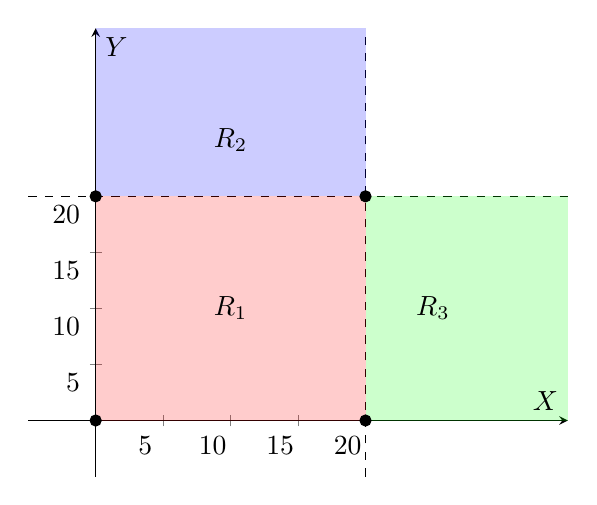
\begin{tikzpicture}
            \begin{axis}[
                axis lines = center,
                xlabel = $X$,
                ylabel = $Y$,
                xmin = -5, xmax = 35,
                ymin = -5, ymax = 35,
                xtick = {0,5,10,15,20},
                ytick = {0,5,10,15,20},
                yticklabel style = {yshift=-1.5ex},
                xticklabel style = {xshift=-1.5ex},
            ]
                \addplot[only marks] coordinates {
                    (0,0) (20,0) (0,20) (20,20)
                };

                % Líneas verticales
                \foreach \x in {20} {
                    \addplot[dashed] coordinates {(\x, -5) (\x, 35)};
                }

                % Líneas horizontales
                \foreach \y in {20} {
                    \addplot[dashed] coordinates {(-5, \y) (35, \y)};
                }                

                % Coloreamos cada una de las zonas
                \fill[red, opacity=0.2] (0,0) -- (20,0) -- (20,20) -- (0,20) -- cycle;
                \fill[blue, opacity=0.2] (0,20) -- (0,35) -- (20,35) -- (20,20) -- cycle;
                \fill[green, opacity=0.2] (20,0) -- (20,20) -- (35,20) -- (35,0) -- cycle;

                % Damos nombres a cada una de las zonas formadas
                \node at (10,10) {$R_1$};
                \node at (10,25) {$R_2$};
                \node at (25,10) {$R_3$};
            \end{axis}
        \end{tikzpicture}
    \end{figure}

    La función de distribución es:
    \begin{equation*}
        F_{(X,Y)}(x, y) = \int_{-\infty}^x \int_{-\infty}^y f(u, v) \, du \, dv
    \end{equation*}

    Estudiemos cada región por separado:
    \begin{itemize}
        \item \ul{Para $x\leq 0$ o $y\leq 0$}:
        
        Tenemos que $f(u, v) = 0$ para $u\leq x$ o $v\leq y$, por lo que:
        \begin{equation*}
            F_{(X,Y)}(x, y) = \int_{-\infty}^x \int_{-\infty}^y f(u, v) \, du \, dv =
            \int_{-\infty}^x \int_{-\infty}^y 0 \, du \, dv = 0.
        \end{equation*}

        \item \ul{Para $0 < x < 20$ y $0 < y < 20$} (región $R_1$):
        
        Tenemos que:
        \begin{equation*}
            F_{(X,Y)}(x, y) = \int_{-\infty}^x \int_{-\infty}^y f(u, v) \, du \, dv =
            \int_{0}^x \int_{0}^y \frac{1}{400} \, du \, dv = \frac{xy}{400}.
        \end{equation*}

        \item \ul{Para $0 < x < 20$ y $y \geq 20$} (región $R_2$):
        
        Tenemos que:
        \begin{equation*}
            F_{(X,Y)}(x, y) = \int_{-\infty}^x \int_{-\infty}^y f(u, v) \, du \, dv =
            \int_{0}^x \int_{0}^{20} \frac{1}{400} \, du \, dv = \frac{20x}{400} = \frac{x}{20}.
        \end{equation*}

        \item \ul{Para $x \geq 20$ y $0 < y < 20$} (región $R_3$):
        
        Tenemos que:
        \begin{equation*}
            F_{(X,Y)}(x, y) = \int_{-\infty}^x \int_{-\infty}^y f(u, v) \, du \, dv =
            \int_{0}^{20} \int_{0}^y \frac{1}{400} \, du \, dv = \frac{20y}{400} = \frac{y}{20}.
        \end{equation*}

        \item \ul{Para $x \geq 20$ y $y \geq 20$}:
        
        Tenemos que:
        \begin{equation*}
            F_{(X,Y)}(x, y) = \int_{-\infty}^x \int_{-\infty}^y f(u, v) \, du \, dv =
            \int_{0}^{20} \int_{0}^{20} \frac{1}{400} \, du \, dv = \frac{400}{400} = 1.
        \end{equation*}
    \end{itemize}

    Por tanto, la función de distribución es:
    \begin{equation*}
        F_{(X,Y)}(x, y) = \begin{cases}
            0, & x\leq 0 \text{ o } y\leq 0, \\
            \frac{xy}{400}, & 0 < x < 20 \text{ y } 0 < y < 20, \\
            \frac{x}{20}, & 0 < x < 20 \text{ y } y\geq 20, \\
            \frac{y}{20}, & x\geq 20 \text{ y } 0 < y < 20, \\
            1, & x\geq 20 \text{ y } y\geq 20.
        \end{cases}
    \end{equation*}

    Buscamos ahora la probabilidad de que en un día se vendan entre naranjas y manzanas, menos de 20 kilogramos. Para ello, buscamos la región del plano que cumple con la condición $X+Y < 20$. Tras representar la recta $y=20-x$,
    nos quedaremos con la región que queda por debajo de esta recta:
    \begin{figure}[H]
        \centering
        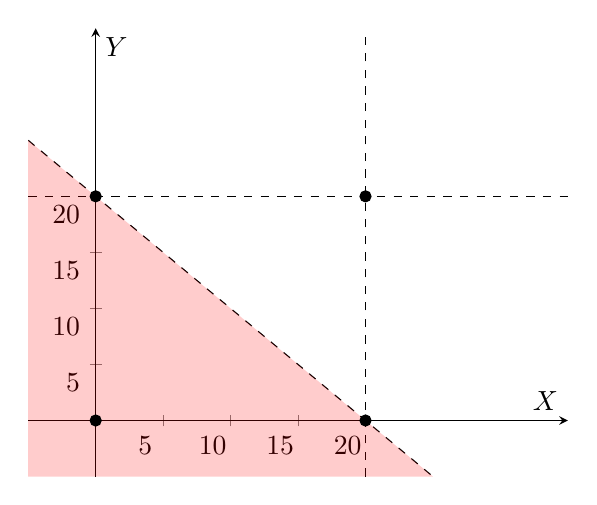
\begin{tikzpicture}
            \begin{axis}[
                axis lines = center,
                xlabel = $X$,
                ylabel = $Y$,
                xmin = -5, xmax = 35,
                ymin = -5, ymax = 35,
                xtick = {0,5,10,15,20},
                ytick = {0,5,10,15,20},
                yticklabel style = {yshift=-1.5ex},
                xticklabel style = {xshift=-1.5ex},
            ]
                \addplot[only marks] coordinates {
                    (0,0) (20,0) (0,20) (20,20)
                };

                % Líneas verticales
                \foreach \x in {20} {
                    \addplot[dashed] coordinates {(\x, -5) (\x, 35)};
                }

                % Líneas horizontales
                \foreach \y in {20} {
                    \addplot[dashed] coordinates {(-5, \y) (35, \y)};
                }

                % Representamos la recta y=20-x
                \addplot[domain=-5:35, samples=2, dashed] {20-x};

                % Coloreamos la región entre el (-5, 25), (25, -5) y (-5,-5)
                \fill[red, opacity=0.2] (-5,25) -- (25,-5) -- (-5,-5) -- cycle;
            \end{axis}
        \end{tikzpicture}
    \end{figure}

    Por tanto, tenemos que $P[X+Y < 20]$ es la integral de la función de densidad en la región coloreada, $R=\{(x,y)\in \mathbb{R}^2; x+y<20\}$:
    \begin{align*}
        P[X+Y < 20] &= \int_{-\infty}^{+\infty} \int_{-\infty}^{20-x} f(x, y) \, dy \, dx = \int_{0}^{20} \int_{0}^{20-x} \frac{1}{400} \, dy \, dx =\\&= \int_{0}^{20} \frac{20-x}{400} \, dx = \frac{1}{400}\left[20x-\frac{x^2}{2}\right]_0^{20} = \frac{1}{400}\left[400-200\right] = \frac{1}{2}.
    \end{align*}
\end{ejercicio}

\begin{ejercicio}
    La renta, $X$, y el consumo, $Y$, de los habitantes de una población, tienen por funciones de densidad
    \[
        f_X(x) = 2-2x; \quad 0 < x < 1; \quad f_{Y\mid X} (y\mid x) = \frac{1}{x}; \quad 0 < y < x.
    \]
    Determinar la función de densidad conjunta del vector aleatorio $(X,Y)$ y la probabilidad de que el consumo sea inferior a la mitad de la renta.\\

    Tenemos que, para $R=\{(x,y)\in \mathbb{R}^2; 0<x<1, 0<y<x\}$, la función de densidad conjunta es:
    \begin{equation*}
        f_{Y\mid X} (y\mid x) = \dfrac{f_{(X,Y)}(x, y)}{f_X(x)} \Longrightarrow f_{(X,Y)}(x, y) = f_X(x) \cdot f_{Y\mid X} (y\mid x) = (2-2x) \cdot \dfrac{1}{x} = \dfrac{2-2x}{x}.
    \end{equation*}

    Tenemos ahora que:
    \begin{align*}
        P[Y < \nicefrac{X}{2}] &= \int_{-\infty}^{+\infty} \int_{-\infty}^{\nicefrac{x}{2}} f_{(X,Y)}(x, y) \, dy \, dx = \int_{0}^{1} \int_{0}^{\nicefrac{x}{2}} \dfrac{2-2x}{x} \, dy \, dx =\\&= \int_{0}^{1} \dfrac{2-2x}{x}\cdot \dfrac{x}{2} \, dx = \int_{0}^{1} 1-x \, dx = \left[x-\dfrac{x^2}{2}\right]_0^1 = 1-\dfrac{1}{2} = \dfrac{1}{2}.
    \end{align*}

    
\end{ejercicio}

\begin{ejercicio}
    Una gasolinera tiene $Y$ miles de litros en su depósito de gasóleo al comienzo de cada semana. A lo largo de una semana se venden $X$ miles de litros del citado combustible, siendo la función de densidad conjunta de $(X,Y)$ :
    \[
        f(x, y) = \frac{1}{8}; \quad 0 < x < y < 4.
    \]
    Se pide:
    \begin{enumerate}
        \item Probar que $f(x, y)$ es función de densidad y obtener la función de distribución.
        
        En primer lugar, vemos que es no negativa. Veamos si es integrable:
        \begin{align*}
            \int_{-\infty}^{+\infty} \int_{-\infty}^{+\infty} f(x, y) \, dx \, dy &= \int_{0}^{4} \int_{x}^{4} \frac{1}{8} \, dy \, dx = \frac{1}{8}\int_{0}^{4} 4-x \, dx =\\&= \frac{1}{8}\left[4x-\frac{x^2}{2}\right]_0^4 = \frac{1}{8}\left[16-8\right] = 1.
        \end{align*}

        Tenemos por tanto que sí se trata de una función de densidad.
        Para obtener la función de distribución, representemos el conjunto en el que la función de densidad es no nula:
        \begin{figure}[H]
            \centering
            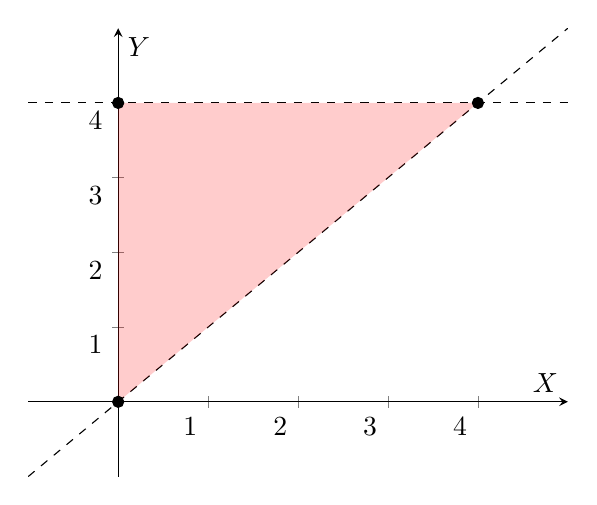
\begin{tikzpicture}
                \begin{axis}[
                    axis lines = center,
                    xlabel = $X$,
                    ylabel = $Y$,
                    xmin = -1, xmax = 5,
                    ymin = -1, ymax = 5,
                    xtick = {0,1,2,3,4},
                    ytick = {0,1,2,3,4},
                    yticklabel style = {yshift=-1.5ex},
                    xticklabel style = {xshift=-1.5ex},
                ]
                    \addplot[only marks] coordinates {
                        (0,0) (0,4) (4,4)
                    };

                    % Líneas horizontales
                    \foreach \y in {4} {
                        \addplot[dashed] coordinates {(-1, \y) (5, \y)};
                    }

                    % Representamos la recta y=x
                    \addplot[domain=-1:5, samples=2, dashed] {x};

                    % Coloreamos la región entre el (0,0), (0,4), (4,4)
                    \fill[red, opacity=0.2] (0,0) -- (0,4) -- (4,4) -- cycle;
                \end{axis}
            \end{tikzpicture}
        \end{figure}

        Para obtener la función de distribución, distinguimos casos:
        \begin{itemize}
            \item \ul{Para $x< 0$ o $y< 0$}:
            \begin{equation*}
                F_{(X,Y)}(x, y) = \int_{-\infty}^x \int_{-\infty}^y f(u, v) \, du \, dv = 0.
            \end{equation*}

            \item \ul{Para $0 < x < y <4$}:
            \begin{align*}
                F_{(X,Y)}(x, y) &= \int_{-\infty}^x \int_{-\infty}^y f(u, v) \, dv \, du = \int_{0}^x \int_{u}^y \frac{1}{8} \, dv \, du = \dfrac{1}{8}\int_{0}^x y-u \, du =\\&= \dfrac{1}{8}\left[yu-\dfrac{u^2}{2}\right]_0^x = \dfrac{1}{8}\left[xy-\dfrac{x^2}{2}\right]
                = \dfrac{2xy-x^2}{16}.
            \end{align*}

            \item \ul{Para $0 < x < 4$ y $y \geq 4$}:
            \begin{align*}
                F_{(X,Y)}(x, y) &= \int_{-\infty}^x \int_{-\infty}^y f(u, v) \, dv \, du =
                \int_0^x \int_u^4 \frac{1}{8} \, dv \, du = \dfrac{1}{8}\int_0^x 4-u \, du =\\&= \dfrac{1}{8}\left[4u-\dfrac{u^2}{2}\right]_0^x = \dfrac{1}{8}\left[4x-\dfrac{x^2}{2}\right] = \dfrac{8x-x^2}{16}.
            \end{align*}

            \item \ul{Para $x\geq y$ y $0\leq y<4$}:
            \begin{align*}
                F_{(X,Y)}(x, y) &= \int_{-\infty}^x \int_{-\infty}^y f(u, v) \, dv \, du =
                \int_0^{y} \int_{0}^v \frac{1}{8} \, du \, dv = \dfrac{1}{8}\int_0^y v \, dv =\\&= \dfrac{1}{8}\left[\dfrac{v^2}{2}\right]_0^y = \dfrac{1}{8}\cdot \dfrac{y^2}{2} = \dfrac{y^2}{16}.
            \end{align*}

            \item \ul{Para $x \geq 4$ y $y \geq 4$}:
            
            Hemos visto anteriormente que $F_{(X,Y)}(x,y) = 1$.
        \end{itemize}

        Por tanto,
        \begin{equation*}
            F_{(X,Y)}(x, y) = \begin{cases}
                0, & x<0 \text{ o } y<0, \\
                \dfrac{2xy-x^2}{16}, & 0 < x < 4 \text{ y } 0 < y < 4, \\
                \dfrac{8x-x^2}{16}, & 0 < x < 4 \text{ y } y\geq 4, \\
                \dfrac{y^2}{16}, & x\geq y \text{ y } 0 \leq y < 4, \\
                1, & x\geq 4 \text{ y } y\geq 4.
            \end{cases}
        \end{equation*}

        

        \item Probabilidad de que en una semana se venda más de la tercera parte de los litros de que se dispone al comienzo de la misma.
        
        En este caso, nos piden calcular $P[X > \nicefrac{Y}{3}]$. Para ello, representamos la recta $y=3x$ y nos quedamos con la región que queda por encima de esta recta:
        \begin{figure}[H]
            \centering
            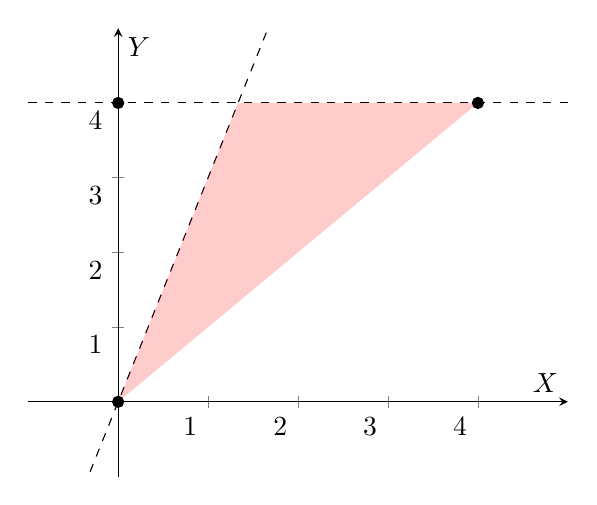
\begin{tikzpicture}
                \begin{axis}[
                    axis lines = center,
                    xlabel = $X$,
                    ylabel = $Y$,
                    xmin = -1, xmax = 5,
                    ymin = -1, ymax = 5,
                    xtick = {0,1,2,3,4},
                    ytick = {0,1,2,3,4},
                    yticklabel style = {yshift=-1.5ex},
                    xticklabel style = {xshift=-1.5ex},
                ]
                    \addplot[only marks] coordinates {
                        (0,0) (0,4) (4,4)
                    };

                    % Líneas horizontales
                    \foreach \y in {4} {
                        \addplot[dashed] coordinates {(-1, \y) (5, \y)};
                    }

                    % Representamos la recta y=3x
                    \addplot[domain=-1:5, samples=2, dashed] {3*x};

                    % Coloreamos la región entre el (0,0), (0,4), (4,4)
                    \fill[red, opacity=0.2] (0,0) -- (4,4) -- (1.333,4) -- cycle;
                \end{axis}
            \end{tikzpicture}
        \end{figure}

        Tenemos que integrar $f(x, y)$ en la región coloreada:
        \begin{align*}
            P[X > \nicefrac{Y}{3}] &=
            \int_{0}^{\nicefrac{4}{3}}
            \int_{x}^{3x} \frac{1}{8} \, dy \, dx + \int_{\nicefrac{4}{3}}^{4}
            \int_{x}^{4} \frac{1}{8} \, dy \, dx =\\&=
            \int_{0}^{\nicefrac{4}{3}} \frac{3x-x}{8} \, dx + \int_{\nicefrac{4}{3}}^{4} \frac{4-x}{8} \, dx = \dfrac{1}{8}\int_{0}^{\nicefrac{4}{3}} 2x \, dx + \dfrac{1}{8}\int_{\nicefrac{4}{3}}^{4} 4-x \, dx =\\&=
            \dfrac{1}{8}\left[x^2\right]_0^{\nicefrac{4}{3}} + \dfrac{1}{8}\left[4x-\dfrac{x^2}{2}\right]_{\nicefrac{4}{3}}^4
            = \dfrac{1}{8}\left[\dfrac{16}{9}\right] + \dfrac{1}{8}\left[16-\dfrac{16}{2}-\dfrac{16}{3}+\dfrac{16}{18}\right]
            =\\&= \dfrac{2}{9} + \dfrac{4}{9} = \dfrac{6}{9} = \dfrac{2}{3}.
        \end{align*}
        \item Si en una semana se han vendido $3.000$ litros de gasóleo, ¿cuál es la probabilidad de que al comienzo de la semana hubiese entre $3.500$ y $3.750$ litros de combustible?\\
        
        En este caso, nos piden:
        \begin{equation*}
            P[3.5 < Y < 3.75 \mid X = 3] = \int_{3.5}^{3.75} f_{Y\mid X=3} (y) \, dy.
        \end{equation*}

        Veamos el valor de $f_{Y\mid X=3} (y)$:
        \begin{equation*}
            f_{Y\mid X=3} (y) = \dfrac{f_{(X,Y)}(3, y)}{f_X(3)}
        \end{equation*}

        Calculemos por tanto la marginal de $X$:
        \begin{equation*}
            f_X(x) = \int_{-\infty}^{+\infty} f(x, y) \, dy = \int_{x}^{4} \dfrac{1}{8} \, dy = \frac{1}{8}\left[y\right]_x^4 = \frac{4-x}{8}
        \end{equation*}

        Por tanto, tenemos que:
        \begin{equation*}
            f_{Y\mid X=3} (y) = \dfrac{f_{(X,Y)}(3, y)}{f_X(3)} = \dfrac{\nicefrac{1}{8}}{\nicefrac{1}{8}} = 1.
        \end{equation*}

        Por tanto, la probabilidad pedida es:
        \begin{equation*}
            P[3.5 < Y < 3.75 \mid X = 3] = \int_{3.5}^{3.75} 1 \, dy = \left[y\right]_{3.5}^{3.75} = 3.75-3.5 = 0.25.
        \end{equation*}

    \end{enumerate}
\end{ejercicio}

\begin{ejercicio}
    Sea $(X,Y)$ un vector aleatorio continuo con función de densidad
    \[
        f(x, y) = k, \quad (x, y) \in R,
    \]
    siendo $R$ el rombo de vértices $(3,0)$; $(0,2)$; $(-3,0)$; $(0,-2)$. Calcular $k$ para que $f$ sea una función de densidad. Hallar las distribuciones marginales y condicionadas.\\

    Representamos en el plano cartesiano el rombo $R$:
    \begin{figure}[H]
        \centering
        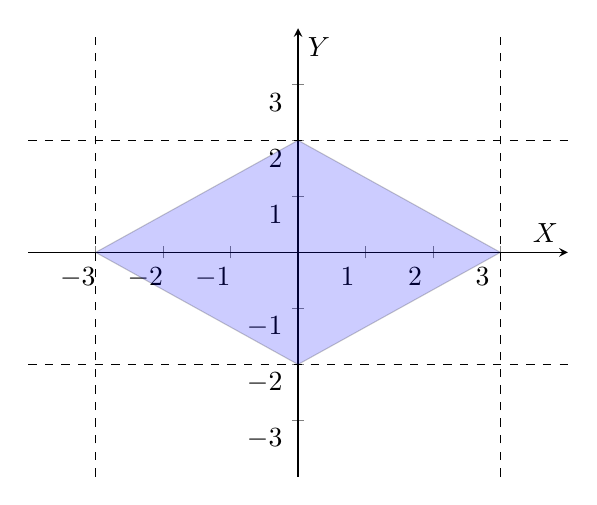
\begin{tikzpicture}
            \begin{axis}[
                axis lines = center,
                xlabel = $X$,
                ylabel = $Y$,
                xmin = -4, xmax = 4,
                ymin = -4, ymax = 4,
                xtick = {-3,-2,-1,0,1,2,3},
                ytick = {-3,-2,-1,0,1,2,3},
                yticklabel style = {yshift=-1.5ex},
                xticklabel style = {xshift=-1.5ex},
            ]
                \addplot[fill=blue, opacity=0.2] coordinates {
                    (3,0) (0,2) (-3,0) (0,-2)
                } --cycle;

                % Líneas horizontales
                \foreach \y in {2,-2} {
                    \addplot[dashed] coordinates {(-4, \y) (4, \y)};
                }

                % Líneas verticales
                \foreach \x in {-3,3} {
                    \addplot[dashed] coordinates {(\x, -4) (\x, 4)};
                }
            \end{axis}
        \end{tikzpicture}
    \end{figure}

    Para que $f$ sea una función de densidad, tenemos que:
    \begin{equation*}
        \int_{-\infty}^{+\infty} \int_{-\infty}^{+\infty} f(x, y) \, dx \, dy = 1.
    \end{equation*}

    Calculamos solo la integral en el primer cuadrante, ya que la función es simétrica. Para ello, calculamos la integral en el triángulo de vértices $(0,0)$; $(3,0)$; $(0,2)$. La recta que une los puntos $(3,0)$ y $(0,2)$ es $y=\nicefrac{-2}{3}x+2$. Por tanto, tenemos:
    \begin{align*}
        1&=\int_{-\infty}^{+\infty} \int_{-\infty}^{+\infty} f(x, y) \, dx \, dy
        = \int_R f(x, y) \, dx \, dy = 4\cdot \int_{0}^{3} \int_{0}^{\nicefrac{-2}{3}\cdot x+2} k \, dy \, dx =\\&= 4k\cdot \int_{0}^{3} \left[-\frac{2}{3}\cdot x+2\right] \, dx = 4k\cdot \left[-\frac{1}{3}\cdot x^2+2x\right]_0^3 = 4k\cdot \left[-\frac{1}{3}\cdot 9+6\right] = 4k\cdot \left[-3+6\right] = 12k.
    \end{align*}

    Por tanto, tenemos que $k=\nicefrac{1}{12}$. En este caso, vemos que además $f_{(X,Y)}$ es no negativa e integrable.\\

    Calculemos ahora la distribución marginal de $X$. Distinguimos:
    \begin{itemize}
        \item \ul{Si $x<-3$ o $x\geq 3$}:
        \begin{equation*}
            f_X(x) = \int_{-\infty}^{+\infty} f(x, y) \, dy = 0.
        \end{equation*}

        \item \ul{Si $-3\leq x<0$}:
    
        En este caso, tenemos que:
        \begin{equation*}
            -\dfrac{2}{3}\cdot x-2 \leq y \leq \dfrac{2}{3}\cdot x+2.
        \end{equation*}

        Por tanto, tenemos:
        \begin{align*}
            f_X(x) &= \int_{-\infty}^{+\infty} f(x, y) \, dy = \int_{\nicefrac{-2}{3}\cdot x-2}^{\nicefrac{2}{3}\cdot x+2} \frac{1}{12} \, dy = \frac{1}{12}\cdot \left[\nicefrac{2}{3}\cdot x+2-\left(\nicefrac{-2}{3}\cdot x-2\right)\right] =\\
            &= \frac{1}{12}\cdot \left[\frac{4}{3}\cdot x+4\right] = \dfrac{x}{9} + \dfrac{1}{3}.
        \end{align*}

        \item \ul{Si $0\leq x<3$}:
        
        En este caso, tenemos que:
        \begin{equation*}
            \frac{2}{3}\cdot x-2 \leq y \leq -\frac{2}{3}\cdot x+2.
        \end{equation*}

        Por tanto, tenemos:
        \begin{align*}
            f_X(x) &= \int_{-\infty}^{+\infty} f(x, y) \, dy = \int_{\nicefrac{2}{3}\cdot x-2}^{\nicefrac{-2}{3}\cdot x+2} \frac{1}{12} \, dy = \frac{1}{12}\cdot \left[\nicefrac{-2}{3}\cdot x+2-\left(\nicefrac{2}{3}\cdot x-2\right)\right] =\\
            &= \frac{1}{12}\cdot \left[-\frac{4}{3}\cdot x+4\right] = -\dfrac{x}{9} + \dfrac{1}{3}.
        \end{align*}
    \end{itemize}

    Por tanto, tenemos que:
    \begin{equation*}
        f_X(x) = \begin{cases}
            0, & x<-3 \text{ o } x\geq 3, \\
            \dfrac{x}{9} + \dfrac{1}{3}, & -3\leq x<0, \\
            -\dfrac{x}{9} + \dfrac{1}{3}, & 0\leq x<3.
        \end{cases}
    \end{equation*}

    Calculemos ahora la distribución marginal de $Y$. Distinguimos:
    \begin{itemize}
        \item \ul{Si $y<-2$ o $y\geq 2$}:
        \begin{equation*}
            f_Y(y) = \int_{-\infty}^{+\infty} f(x, y) \, dx = 0.
        \end{equation*}

        \item \ul{Si $-2\leq y<0$}:
    
        En este caso, tenemos que:
        \begin{equation*}
            -\frac{3}{2}\cdot y-3 \leq x \leq \frac{3}{2}\cdot y+3
        \end{equation*}

        Por tanto, tenemos:
        \begin{align*}
            f_Y(y) &= \int_{-\infty}^{+\infty} f(x, y) \, dx =
            \int_{\nicefrac{-3}{2}\cdot y-3}^{\nicefrac{3}{2}\cdot y+3} \frac{1}{12} \, dx = \frac{1}{12}\cdot \left[\nicefrac{3}{2}\cdot y+3-\left(\nicefrac{-3}{2}\cdot y-3\right)\right] =\\
            &= \dfrac{\nicefrac{y}{2}+1}{2} = \dfrac{y}{4} + \dfrac{1}{2}.
        \end{align*}

        \item \ul{Si $0\leq y<2$}:
        
        En este caso, tenemos que:
        \begin{equation*}
            \frac{3}{2}\cdot y-3 \leq x \leq -\frac{3}{2}\cdot y+3
        \end{equation*}

        Por tanto, tenemos:
        \begin{align*}
            f_Y(y) &= \int_{-\infty}^{+\infty} f(x, y) \, dx =
            \int_{\nicefrac{3}{2}\cdot y-3}^{\nicefrac{-3}{2}\cdot y+3} \frac{1}{12} \, dx = \frac{1}{12}\cdot \left[\nicefrac{-3}{2}\cdot y+3-\left(\nicefrac{3}{2}\cdot y-3\right)\right] =\\
            &= \dfrac{\nicefrac{-y}{2}+1}{2} = -\dfrac{y}{4} + \dfrac{1}{2}.
        \end{align*}
    \end{itemize}

    Por tanto, tenemos que:
    \begin{equation*}
        f_Y(y) = \begin{cases}
            0, & y<-2 \text{ o } y\geq 2, \\
            \dfrac{y}{4} + \dfrac{1}{2}, & -2\leq y<0, \\
            -\dfrac{y}{4} + \dfrac{1}{2}, & 0\leq y<2.
        \end{cases}
    \end{equation*}

    Calculemos ahora las distribuciones condicionadas.
    Dado $x^\ast\in \left]-3,3\right[$, tenemos:
    \begin{equation*}
        f_{Y\mid X=x^\ast} (y) = \dfrac{f_{(X,Y)}(x^\ast, y)}{f_X(x^\ast)}
        = \begin{cases}
            \dfrac{1}{12}\cdot \dfrac{1}{\nicefrac{x}{9} + \nicefrac{1}{3}}, & -3< x^\ast<0, \\
            \dfrac{1}{12}\cdot \dfrac{1}{\nicefrac{-x}{9} + \nicefrac{1}{3}}, & 0\leq x^\ast<3.
        \end{cases}
    \end{equation*}

    Por otro lado, dado $y^\ast\in \left]-2,2\right[$, tenemos que:
    \begin{equation*}
        f_{X\mid Y=y^\ast} (x) = \dfrac{f_{(X,Y)}(x, y^\ast)}{f_Y(y^\ast)}
        = \begin{cases}
            \dfrac{1}{12}\cdot \dfrac{1}{\nicefrac{y}{4} + \nicefrac{1}{2}}, & -2< y^\ast<0, \\
            \dfrac{1}{12}\cdot \dfrac{1}{\nicefrac{-y}{4} + \nicefrac{1}{2}}, & 0\leq y^\ast<2.
        \end{cases}
    \end{equation*}
\end{ejercicio}

\begin{ejercicio}
    Sea $(X,Y)$ un vector aleatorio continuo con función de densidad
    \[
        f(x, y) = k, \quad x^2 \leq y \leq 1,
    \]
    anulándose fuera del recinto indicado.
    \begin{enumerate}
        \item Hallar la constante $k$ para que $f$ sea una función de densidad.
        
        Representamos en el plano cartesiano el recinto en el que la función de densidad es no nula:
        \begin{figure}[H]
            \centering
            \begin{tikzpicture}
                \begin{axis}[
                    axis lines = center,
                    xlabel = $X$,
                    ylabel = $Y$,
                    xmin = -2, xmax = 2,
                    ymin = -0.5, ymax = 2,
                    xtick = {-1,0,1},
                    ytick = {-1,0,1},
                    yticklabel style = {yshift=-1.5ex},
                    xticklabel style = {xshift=-1.5ex},
                ]
                
                    % Dibuja la curva de y = x^2
                    \addplot [name path=A, blue, thick, forget plot, samples=70] {x^2};
                    
                    % Dibuja la línea horizontal en y=2
                    \addplot [name path=B, dashed, thick, forget plot] {1};
                
                    % Rellena el área bajo la curva entre x=0 y x=2
                    \addplot [
                        thick,
                        color=orange,
                        fill=orange,
                        fill opacity=0.4
                    ]
                    fill between [
                        of=A and B,
                        soft clip={domain=-1:1},
                    ];

                    % Coloreamos el área por debajo de A
                    \addplot [name path=C] {0};
                    \addplot [
                        thick,
                        color=red,
                        fill=red,
                        fill opacity=0.4
                    ]
                    fill between [
                        of=A and C,
                        soft clip={domain=-2:0},
                    ];

                    % Coloreamos el área por debajo de y=0
                    \addplot[fill=red, opacity=0.4] coordinates {
                        (-2, 0) (2,0) (2, -0.5) (-2, -0.5)
                    } --cycle;

                    % Coloreamos el área entre A y la recta x=-1
                    \addplot[name path=D] {3};
                    \addplot [
                        thick,
                        color=red,
                        fill=red,
                        fill opacity=0.4
                    ]
                    fill between [
                        of=D and A,
                        soft clip={domain=-2:-1},
                    ];

                    \addplot[fill=blue, opacity=0.2] coordinates {
                        (-1, 2) (-1, 1) (1,1) (1,2)
                    } --cycle;
                    
                    % Coloramos la zona R_4
                    \addplot [
                        thick,
                        color=green,
                        fill=green,
                        fill opacity=0.2
                    ]
                    fill between [
                        of=A and C,
                        soft clip={domain=0:1},
                    ];
                    \addplot[fill=green, opacity=0.2] coordinates {
                        (1,0) (1,1) (2,1) (2,0)
                    } --cycle;

                    \addplot[fill=olive, opacity=0.2] coordinates {
                        (1,1) (1,2) (2,2) (2,1)
                    } --cycle;


                    % Rectas verticales
                    \foreach \x in {-1,1} {
                        \addplot[dashed] coordinates {(\x, -0.5) (\x, 2)};
                    }

                    % Marcamos las zonas
                    \node at (-1.5, 0.5) {$R_1$};
                    \node at (0.3, 0.5) {$R_2$};
                    \node at (0.5, 1.5) {$R_3$};
                    \node at (1.5, 0.5) {$R_4$};
                    \node at (1.5, 1.5) {$R_5$};

                \end{axis}
            \end{tikzpicture}
        \end{figure}

        Para que $f$ sea una función de densidad, tenemos que:
        \begin{equation*}
            \int_{-\infty}^{+\infty} \int_{-\infty}^{+\infty} f(x, y) \, dx \, dy = 1.
        \end{equation*}

        Tenemos por tanto que:
        \begin{align*}
            1&=\int_{-\infty}^{+\infty} \int_{-\infty}^{+\infty} f(x, y) \, dx \, dy
            = \int_{-1}^{1} \int_{x^2}^{1} k \, dy \, dx = k\cdot \int_{-1}^{1} \left[y\right]_{x^2}^{1} \, dx = k\cdot \int_{-1}^{1} 1-x^2 \, dx =\\&= k\cdot \left[x-\dfrac{x^3}{3}\right]_{-1}^{1} = k\cdot \left[1-\dfrac{1}{3}-\left(-1+\dfrac{1}{3}\right)\right] = k\cdot \left[2-\dfrac{2}{3}\right] = \dfrac{4}{3}k
        \end{align*}
        Por tanto, tenemos que $k=\nicefrac{3}{4}$. En este caso, vemos que además $f_{(X,Y)}$ es no negativa e integrable.

        \item Calcular la función de distribución de probabilidad.
        
        Distinguimos casos:
        \begin{itemize}
            \item \ul{Si $x\leq -1$ \quad o \quad $y\leq 0$ \quad o \quad $x\in \left]-1,0\right[$ \text{ y } $y\leq x^2$} (zona $R_1$):
            \begin{equation*}
                F_{(X,Y)}(x, y) = \int_{-\infty}^x \int_{-\infty}^y f(u, v) \, du \, dv = 0.
            \end{equation*}

            \item \ul{Si $x^2\leq y\leq 1$} (zona $R_2$):
            \begin{align*}
                F_{(X,Y)}(x, y) &= \int_{-\infty}^x \int_{-\infty}^y f(u, v) \, dv \, du = \int_{-\sqrt{y}}^x \int_{u^2}^y \frac{3}{4} \, dv \, du = \frac{3}{4}\int_{-\sqrt{y}}^x \left[y-u^2\right] \, du =\\&= \frac{3}{4}\left[yu-\dfrac{u^3}{3}\right]_{-\sqrt{y}}^x = \frac{3}{4}\left[xy-\dfrac{x^3}{3}+y\sqrt{y}-\dfrac{y^{\nicefrac{3}{2}}}{3}\right] =\\
                &= \frac{3}{4}\left[xy-\dfrac{x^3}{3}+\dfrac{2}{3}\cdot y\sqrt{y}\right].
            \end{align*}

            \item \ul{Si $y\geq 1$ y $x\in \left]-1,1\right[$} (zona $R_3$):
            \begin{align*}
                F_{(X,Y)}(x, y) &= \int_{-\infty}^x \int_{-\infty}^y f(u, v) \, dv \, du = \int_{-1}^x \int_{u^2}^1 \frac{3}{4} \, dv \, du = \frac{3}{4}\int_{-1}^x \left[1-u^2\right] \, du =\\&= \frac{3}{4}\left[u-\dfrac{u^3}{3}\right]_{-1}^x = \frac{3}{4}\left[x-\dfrac{x^3}{3}+1-\dfrac{1}{3}\right] = \frac{3}{4}\left[x-\dfrac{x^3}{3}+\dfrac{2}{3}\right].
            \end{align*}

            \item \ul{Si $x\in \left]0,1\right[$ \text{ y } $0\leq y\leq x^2$ \quad o \quad $x\in \left]1,+\infty\right[$ \text{ y } $y\in ]0,1[$} (zona $R_4$):
            \begin{align*}
                F_{(X,Y)}(x, y) &= \int_{-\infty}^x \int_{-\infty}^y f(u, v) \, dv \, du = \int_{-\sqrt{y}}^{\sqrt{y}} \int_{u^2}^y \frac{3}{4} \, dv \, du = \frac{3}{4}\int_{-\sqrt{y}}^{\sqrt{y}} \left[y-u^2\right] \, du =\\&= \frac{3}{4}\left[yu-\dfrac{u^3}{3}\right]_{-\sqrt{y}}^{\sqrt{y}} = \frac{3}{4}\left[y\sqrt{y}-\dfrac{y^{\nicefrac{3}{2}}}{3}+y\sqrt{y}-\dfrac{y^{\nicefrac{3}{2}}}{3}\right] = y\sqrt{y}
            \end{align*}

            \item \ul{Si $x\geq 1$ y $y\geq 1$} (zona $R_5$):
            \begin{equation*}
                F_{(X,Y)}(x, y) = 1.
            \end{equation*}
        \end{itemize}

        Por tanto, tenemos que:
        \begin{equation*}
            F_{(X,Y)}(x, y) = \begin{cases}
                0, & x\leq -1 \text{ o } y\leq 0 \text{ o } x\in \left]-1,0\right[ \text{ y } y\leq x^2, \\
                \dfrac{3}{4}\left[xy-\dfrac{x^3}{3}+\dfrac{2}{3}\cdot y\sqrt{y}\right], & x^2\leq y\leq 1, \\
                \dfrac{3}{4}\left[x-\dfrac{x^3}{3}+\dfrac{2}{3}\right], & y\geq 1 \text{ y } x\in \left]-1,1\right[, \\
                y\sqrt{y}, & x\in \left]0,1\right[ \text{ y } 0\leq y\leq x^2 \text{ o } x>1\text{ y } y\in ]0,1[, \\
                1, & x\geq 1 \text{ y } y\geq 1.
            \end{cases}
        \end{equation*}

        \item Calcular $P(X \geq Y)$.
        
        Para calcular $P(X \geq Y)$, representamos la recta $y=x$ y nos quedamos con la región que queda por debajo de esta recta. Tenemos entonces que:
        \begin{align*}
            P(X \geq Y) &= \int_{0}^{1} \int_{x^2}^{x} \dfrac{3}{4} \, dy \, dx = \dfrac{3}{4}\int_{0}^{1} \left[x-x^2\right]\, dx = 
            \dfrac{3}{4}\left[\dfrac{x^2}{2} -\dfrac{x^3}{3}\right]_0^1 =\\&= \dfrac{3}{4}\left[\dfrac{1}{2}-\dfrac{1}{3}\right] = \dfrac{3}{4}\left[\dfrac{3-2}{6}\right] = \dfrac{3}{4}\left[\dfrac{1}{6}\right] = \dfrac{1}{8}.
        \end{align*}
        \item Calcular las distribuciones marginales.
        
        Para $x\in \left]-1,1\right[$, tenemos que:
        \begin{align*}
            f_X(x) &= \int_{-\infty}^{+\infty} f(x, y) \, dy = \int_{x^2}^{1} \dfrac{3}{4} \, dy = \dfrac{3}{4}\left[y\right]_{x^2}^1 = \dfrac{3}{4}\left[1-x^2\right].
        \end{align*}

        Para $y\in \left]0,1\right[$, tenemos que:
        \begin{align*}
            f_Y(y) &= \int_{-\infty}^{+\infty} f(x, y) \, dx = \int_{-\sqrt{y}}^{\sqrt{y}} \dfrac{3}{4} \, dx = \dfrac{3}{4}\left[x\right]_{-\sqrt{y}}^{\sqrt{y}} = \dfrac{3}{4}\left[\sqrt{y}+\sqrt{y}\right] = \dfrac{3}{2}\sqrt{y}.
        \end{align*}
        \item Calcular las distribuciones condicionadas.
        
        Dado $x^\ast\in \left]-1,1\right[$, tenemos que:
        \begin{equation*}
            f_{Y\mid X=x^\ast} (y) = \dfrac{f_{(X,Y)}(x^\ast, y)}{f_X(x^\ast)} = \dfrac{\nicefrac{3}{4}}{\nicefrac{3}{4}\left[1-(x^\ast)^2\right]} = \dfrac{1}{1-(x^\ast)^2}.
        \end{equation*}

        Dado $y^\ast\in \left]0,1\right[$, tenemos que:
        \begin{equation*}
            f_{X\mid Y=y^\ast} (x) = \dfrac{f_{(X,Y)}(x, y^\ast)}{f_Y(y^\ast)} = \dfrac{\nicefrac{3}{4}}{\nicefrac{3}{2}\sqrt{y^\ast}} = \dfrac{1}{2\sqrt{y^\ast}}.
        \end{equation*}
    \end{enumerate}

\end{ejercicio}

\begin{ejercicio}
    Sea $k\in \bb{R}$. Consideramos la función de densidad de probabilidad
    \[
        f(x, y) = \begin{cases}
            k\left[\frac{xy}{2}+1\right], & 0 < x < 1, -1 < y < 1, \\
            0, & \text{en otro caso}.
        \end{cases}
    \]
    Calcular:
    \begin{enumerate}
        \item La constante $k$ para que $f$ sea una función de densidad.
        
        Para que $f$ sea una función de densidad, tenemos que:
        \begin{equation*}
            \int_{-\infty}^{+\infty} \int_{-\infty}^{+\infty} f(x, y) \, dx \, dy = 1.
        \end{equation*}

        Tenemos por tanto que:
        \begin{align*}
            1&=\int_{-\infty}^{+\infty} \int_{-\infty}^{+\infty} f(x, y) \, dx \, dy
            = \int_{-1}^{1} \int_{0}^{1} k\left[\frac{xy}{2}+1\right] \, dx \, dy = k\int_{-1}^{1} \left[\dfrac{yx^2}{4}+x\right]_0^1
            =\\&= k\int_{-1}^{1} \left[\dfrac{y}{4}+1\right] \, dy = k\left[\dfrac{y^2}{8}+y\right]_{-1}^1 = k\left[\dfrac{1}{8}+1-\left(\dfrac{1}{8}-1\right)\right] = 2k \Longrightarrow k = \dfrac{1}{2}.
        \end{align*}

        Veamos ahora que, para dicho valor de $k$, $f$ es no negativa. Para ello, tenemos que:
        \begin{equation*}
            f(x, y) \geq 0 \Longleftrightarrow xy>-2 \Longleftrightarrow y>\dfrac{-2}{x}
        \end{equation*}
        Esto último es cierto, ya que $x\in ]0,1[$ e $y\in ]-1,1[$. Por tanto, $f$ es no negativa. Además, es integrable, por lo que $f$ es una función de densidad.

        \item La función de distribución de probabilidad.
        
        Representamos en el plano cartesiano la región en la que la función de densidad es no nula:
        \begin{figure}[H]
            \centering
            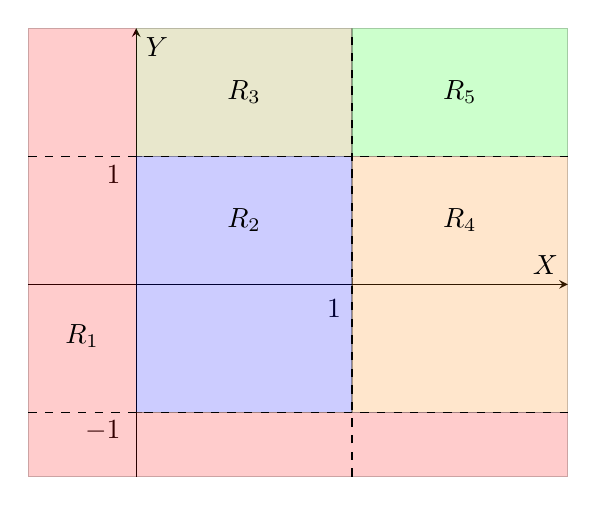
\begin{tikzpicture}
                \begin{axis}[
                    axis lines = center,
                    xlabel = $X$,
                    ylabel = $Y$,
                    xmin = -0.5, xmax = 2,
                    ymin = -1.5, ymax = 2,
                    xtick = {-1,0,1},
                    ytick = {-1,0,1},
                    yticklabel style = {yshift=-1.5ex},
                    xticklabel style = {xshift=-1.5ex},
                ]
                    \addplot[fill=red, opacity=0.2] coordinates {
                        (-0.5, -1.5) (-0.5,2) (0,2) (0,-1.5)
                    } --cycle;
                    \addplot[fill=red, opacity=0.2] coordinates {
                        (0, -1.5) (0, -1) (2,-1) (2,-1.5)
                    } --cycle;
                    \node at (-0.25, -0.4) {$R_1$};

                    \addplot[fill=blue, opacity=0.2] coordinates {
                        (0, -1) (1,-1) (1,1) (0,1)
                    } --cycle;
                    \node at (0.5, 0.5) {$R_2$};

                    \addplot[fill=olive, opacity=0.2] coordinates {
                        (0, 1) (1,1) (1,2) (0,2)
                    } --cycle;
                    \node at (0.5, 1.5) {$R_3$};

                    \addplot[fill=orange, opacity=0.2] coordinates {
                        (1,-1) (2,-1) (2,1) (1,1)
                    } --cycle;
                    \node at (1.5, 0.5) {$R_4$};

                    \addplot[fill=green, opacity=0.2] coordinates {
                        (1,1) (2,1) (2,2) (1,2)
                    } --cycle;
                    \node at (1.5, 1.5) {$R_5$};

                    % Líneas verticales
                    \foreach \x in {1} {
                        \addplot[dashed] coordinates {(\x, -1.5) (\x, 2)};
                    }

                    % Líneas horizontales
                    \foreach \y in {-1,1} {
                        \addplot[dashed] coordinates {(-0.5, \y) (2, \y)};
                    }
                \end{axis}
            \end{tikzpicture}
        \end{figure}

        Distinguimos casos:
        \begin{itemize}
            \item \ul{Si $x\leq 0 \qquad \text{o} \qquad y\leq -1$} (zona $R_1$):
            \begin{equation*}
                F_{(X,Y)}(x, y) = \int_{-\infty}^x \int_{-\infty}^y
                f(u, v) \, du \, dv = 0.
            \end{equation*}

            \item \ul{Si $x\in \left]0,1\right[ \text{ y } y\in \left]-1,1\right[$} (zona $R_2$):
            \begin{align*}
                F_{(X,Y)}(x, y) &= \int_{-\infty}^x \int_{-\infty}^y
                f(u, v) \, du \, dv = \int_{0}^x \int_{-1}^y
                \dfrac{1}{2}\left[\dfrac{uv}{2}+1\right] \, dv \, du =\\&= \int_{0}^x \left[\dfrac{uv^2}{8}+\frac{v}{2}\right]_{-1}^y \, du =
                \int_{0}^x \dfrac{uy^2}{8}+\frac{y}{2}-\dfrac{u}{8}+\dfrac{1}{2} \, du =\\&= \left[\dfrac{u^2y^2}{16}+\frac{y}{2}u-\dfrac{u^2}{16}+\dfrac{u}{2}\right]_0^x = \dfrac{x^2y^2}{16}+\frac{xy}{2}-\dfrac{x^2}{16}+\dfrac{x}{2}.
            \end{align*}

            \item \ul{Si $x\in \left]0,1\right[ \text{ y } y\geq 1$} (zona $R_3$):
            \begin{align*}
                F_{(X,Y)}(x, y) &= \int_{-\infty}^x \int_{-\infty}^y
                f(u, v) \, du \, dv = \int_{0}^x \int_{-1}^1
                \dfrac{1}{2}\left[\dfrac{uv}{2}+1\right] \, dv \, du =\\&= \int_{0}^x \left[\dfrac{uv^2}{8}+\frac{v}{2}\right]_{-1}^1 \, du =
                \int_{0}^x \dfrac{u}{8}+\dfrac{1}{2} - \left(\dfrac{u}{8}-\dfrac{1}{2}\right) \, du = \int_{0}^x 1 \, du = x.
            \end{align*}

            \item \ul{Si $y\in \left]-1,1\right[$ \text{ y } $x\geq 1$} (zona $R_4$):
            \begin{align*}
                F_{(X,Y)}(x, y) &= \int_{-\infty}^x \int_{-\infty}^y
                f(u, v) \, du \, dv = \int_{0}^1 \int_{-1}^y
                \dfrac{1}{2}\left[\dfrac{uv}{2}+1\right] \, dv \, du =\\&=
                \int_{0}^1 \left[\dfrac{uv^2}{8}+\frac{v}{2}\right]_{-1}^y \, du =
                \int_{0}^1 \dfrac{uy^2}{8}+\frac{y}{2}-\dfrac{u}{8}+\dfrac{1}{2} \, du =\\&=
                \left[\dfrac{u^2y^2}{16}+\frac{y}{2}u-\dfrac{u^2}{16}+\dfrac{u}{2}\right]_0^1 = \dfrac{y^2}{16}+\frac{y}{2}+\dfrac{7}{16}
            \end{align*}

            \item \ul{Si $y\geq 1$ \text{ y } $x\geq 1$} (zona $R_5$):
            \begin{equation*}
                F_{(X,Y)}(x, y) = 1.
            \end{equation*}
        \end{itemize}

        Por tanto, tenemos que:
        \begin{equation*}
            F_{(X,Y)}(x, y) = \begin{cases}
                0, & x\leq 0 \text{ o } y\leq -1, \\
                \dfrac{x^2y^2}{16}+\dfrac{xy}{2}-\dfrac{x^2}{16}+\dfrac{x}{2}, & x\in \left]0,1\right[ \text{ y } y\in \left]-1,1\right[, \\
                x, & x\in \left]0,1\right[ \text{ y } y\geq 1,\\
                \dfrac{y^2}{16}+\dfrac{y}{2}+\dfrac{7}{16}, & y\in \left]-1,1\right[ \text{ y } x\geq 1, \\
                1, & y\geq 1 \text{ y } x\geq 1.
            \end{cases}
        \end{equation*}
            

        \item Las distribuciones marginales.
        
        Para $x\in \left]0,1\right[$, tenemos que:
        \begin{align*}
            f_X(x) &= \int_{-\infty}^{+\infty} f(x, y) \, dy = \int_{-1}^{1} \dfrac{1}{2}\left[\dfrac{xy}{2}+1\right] \, dy = \dfrac{1}{2}\left[\dfrac{xy^2}{4}+y\right]_{-1}^1 = \dfrac{1}{2}\left[\dfrac{x}{4}+1-\dfrac{x}{4}+1\right] = 1
        \end{align*}

        Para $y\in \left]-1,1\right[$, tenemos que:
        \begin{align*}
            f_Y(y) &= \int_{-\infty}^{+\infty} f(x, y) \, dx = \int_{0}^{1} \dfrac{1}{2}\left[\dfrac{xy}{2}+1\right] \, dx = \dfrac{1}{2}\left[\dfrac{x^2y}{4}+x\right]_{0}^1 = \dfrac{1}{2}\left[\dfrac{y}{4}+1\right]
        \end{align*}
    \end{enumerate}
\end{ejercicio}

\begin{ejercicio}
    Sea $(X,Y)$ un vector aleatorio bidimensional continuo, con función de densidad de probabilidad
    \[
        f(x, y) = \begin{cases}
            k, & 0 < x + y < 1, |y| < 1, 0 < x < 1, \\
            0, & \text{en otro caso}.
        \end{cases}
    \]
    Responder a los siguientes apartados:
    \begin{enumerate}
        \item Hallar la constante $k$ para que $f$ sea una función de densidad de probabilidad.
        
        Para que $f$ sea una función de densidad, tenemos que:
        \begin{equation*}
            \int_{-\infty}^{+\infty} \int_{-\infty}^{+\infty} f(x, y) \, dx \, dy = 1.
        \end{equation*}

        Tenemos por tanto que:
        \begin{align*}
            1&=\int_{0}^{1} \int_{-x}^{1-x} k \, dx \, dy = k\int_{0}^{1} \left[y\right]_{-x}^{1-x} \, dx = k\int_{0}^{1} 1-x+x \, dx = k\int_{0}^{1} 1 \, dx = k
        \end{align*}

        Por tanto, tenemos que $k=1$. En este caso, vemos que además $f_{(X,Y)}$ es no negativa e integrable.

        \item Calcular la función de distribución de probabilidad.
        
        Dividimos el plano cartesiano en las distintas regiones:
        \begin{figure}[H]
            \centering
            \begin{tikzpicture}
                \begin{axis}[
                    axis lines = center,
                    xlabel = $X$,
                    ylabel = $Y$,
                    xmin = -1.5, xmax = 2,
                    ymin = -1.5, ymax = 2,
                    xtick = {-1,0,1},
                    ytick = {-1,0,1},
                    yticklabel style = {yshift=-1.5ex},
                    xticklabel style = {xshift=-1.5ex},
                ]
                    % Recta x+y=0
                    \addplot [name path=A, blue, thick, forget plot, samples=2] {-x};

                    % Recta x+y=1
                    \addplot [name path=B, blue, thick, forget plot, samples=2] {1-x};

                    % R1: Triangulo (0,1), (1,0), (0,0)
                    \addplot[fill=red, opacity=0.2] coordinates {
                        (0, 0) (1,0) (0,1)
                    } --cycle;
                    \node at (0.25, 0.25) {$R_1$};

                    % R2: Triangulo (1,0), (0,0), (1,-1)
                    \addplot[fill=blue, opacity=0.2] coordinates {
                        (1, 0) (0,0) (1,-1)
                    } --cycle;
                    \node at (0.75, -0.25) {$R_2$};

                    % R3: y<=0 y triángulo (0,0), (5,-5), (0,-5)
                    \addplot[fill=olive, opacity=0.2] coordinates {
                        (0, 0) (5,-5) (0,-5)
                    } --cycle;
                    \node at (0.5, -1) {$R_3$};
                    \addplot[fill=olive, opacity=0.2] coordinates {
                        (0, 5) (-5,5) (-5,-5) (0,-5)
                    } --cycle;
                    \addplot[fill=olive, opacity=0.2] coordinates {
                        (1, -1) (5,-1) (5, -5)
                    } --cycle;

                    % R4: Triangulo (1,0), (1,11), (0,1)
                    \addplot[fill=orange, opacity=0.2] coordinates {
                        (1, 0) (1,1) (0,1)
                    } --cycle;
                    \node at (0.75, 0.5) {$R_4$};

                    % R5: (0,1), (0,5), (1,5) y (1,1)
                    \addplot[fill=green, opacity=0.2] coordinates {
                        (0, 1) (0,5) (1,5) (1,1)
                    } --cycle;
                    \node at (0.5, 1.3) {$R_5$};

                    % R6: (1,1), (5,1), (5,0) y (1,0)
                    \addplot[fill=gray, opacity=0.2] coordinates {
                        (1, 1) (5,1) (5,0) (1,0)
                    } --cycle;
                    \node at (1.5, 0.5) {$R_6$};

                    % R7: (1,0), (1,-1), (5,-1) y (5,0)
                    \addplot[fill=yellow, opacity=0.2] coordinates {
                        (1, 0) (1,-1) (5,-1) (5,0)
                    } --cycle;
                    \node at (1.5, -0.5) {$R_7$};

                    % R8: (1,1), (1,5), (5,5) y (5,1)
                    \addplot[fill=pink, opacity=0.2] coordinates {
                        (1, 1) (1,5) (5,5) (5,1)
                    } --cycle;
                    \node at (1.5, 1.5) {$R_8$};                
                \end{axis}
            \end{tikzpicture}
        \end{figure}

        Distinguimos casos:
        \begin{itemize}
            \item \ul{Si $x\leq 0$ \quad o \quad $x+y\leq 0$} (zona $R_3$):
            \begin{equation*}
                F_{(X,Y)}(x, y) = \int_{-\infty}^x \int_{-\infty}^y f(u, v) \, du \, dv = 0.
            \end{equation*}

            \item \ul{Si $x\in \left]0,1\right[$ \quad y \quad $y\in \left]0,1\right[$ \quad y \quad $x+y\leq 1$} (zona $R_1$):
            \begin{align*}
                F_{(X,Y)}(x, y) &= \int_{-\infty}^x \int_{-\infty}^y f(u, v) \, dv \, du = \int_{0}^x \int_{-u}^y 1 \, dv \, du = \int_{0}^x \left[v\right]_{-u}^y \, du
                =\\&= \int_{0}^x y+u \, du = \left[yu+\dfrac{u^2}{2}\right]_0^x = yx+\dfrac{x^2}{2}.
            \end{align*}

            \item \ul{Si $x\in \left]0,1\right[$ \quad y \quad $y\in \left]-1,0\right[$ \quad y \quad $x+y\geq 0$} (zona $R_2$):
            \begin{align*}
                F_{(X,Y)}(x, y) &= \int_{-\infty}^x \int_{-\infty}^y f(u, v) \, du \, dv = \int_{-y}^x \int_{-u}^y 1 \, dv \, du = \int_{-y}^x \left[v\right]_{-u}^y \, du
                =\\&= \int_{-y}^x y+u \, du = \left[yu+\dfrac{u^2}{2}\right]_{-y}^x = xy+\dfrac{x^2}{2}-y(-y)-\dfrac{y^2}{2} = yx+\dfrac{x^2+y^2}{2}.
            \end{align*}

            \item \ul{Si $x\in \left]0,1\right[$ \quad y \quad $y\in \left]0,1\right[$ \quad y \quad $x+y\geq 1$} (zona $R_4$):
            \begin{align*}
                F_{(X,Y)}(x, y) &= \int_{-\infty}^x \int_{-\infty}^y f(u, v) \, du \, dv
                =\\&= \int_{0}^{1-y} \int_{0}^y 1 \, dv \, du
                + \int_{1-y}^x \int_{0}^{1-u} 1 \, dv \, du
                + \int_{0}^{x} \int_{-u}^0 1 \, dv \, du
                =\\&= \int_{0}^{1-y} y  \, du
                + \int_{1-y}^x 1-u \, du
                + \int_{0}^{x} u\, du
                =\\&= \left[yu\right]_0^{1-y}
                + \left[u-\dfrac{u^2}{2}\right]_{1-y}^x
                + \left[\dfrac{u^2}{2}\right]_0^x
                =\\&= y(1-y)+\left(x-\cancel{\dfrac{x^2}{2}}\right)-\left(1-y-\dfrac{(1-y)^2}{2}\right)+\cancel{\dfrac{x^2}{2}}
                =\\&= y-y^2+x-1+y+\dfrac{(1-y)^2}{2}
                = -(1-y)^2+x +\dfrac{(1-y)^2}{2}
                =\\&= x -\dfrac{(1-y)^2}{2}
            \end{align*}

            \item \ul{Si $x\in \left]0,1\right[$ \quad y \quad $y\in \left]1,\infty\right[$} (zona $R_5$):
            \begin{align*}
                F_{(X,Y)}(x, y) &= \int_{-\infty}^x \int_{-\infty}^y f(u, v) \, du \, dv
                = \int_{0}^{x} \int_{-u}^{1-u} 1 \, dv \, du
                =\\&= \int_{0}^{x} \left[v\right]_{-u}^{1-u} \, du
                = \int_{0}^{x} 1-u+u \, du
                = \int_{0}^{x} 1 \, du = x.
            \end{align*}

            \item \ul{Si $x\in \left]1,\infty\right[$ \quad y \quad $y\in \left]0,1\right[$} (zona $R_6$):
            \begin{align*}
                F_{(X,Y)}(x, y) &= \int_{-\infty}^x \int_{-\infty}^y f(u, v) \, du \, dv
                =\\&= \int_{0}^{1} \int_{-u}^{0} 1 \, dv \, du
                + \int_{0}^{1-y} \int_{0}^{y} 1 \, dv \, du
                + \int_{1-y}^{1} \int_{0}^{1-u} 1 \, dv \, du
                =\\&= \int_{0}^{1} u \, du
                + \int_{0}^{1-y} y \, du
                + \int_{1-y}^{1} 1-u \, du
                =\\&= \left[\dfrac{u^2}{2}\right]_0^1
                + \left[yu\right]_0^{1-y}
                + \left[u-\dfrac{u^2}{2}\right]_{1-y}^1
                =\\&= \cancel{\dfrac{1}{2}}+y(1-y)+1-\cancel{\dfrac{1}{2}}-\left[1-y-\dfrac{(1-y)^2}{2}\right]
                =\\&= y-y^2+y +\dfrac{(1-y)^2}{2}
                = 1-\dfrac{(1-y)^2}{2}
            \end{align*}
        \end{itemize}
    \end{enumerate}
\end{ejercicio}

\begin{ejercicio}
    Sea $(X,Y)$ un vector aleatorio bidimensional continuo, con distribución de probabilidad uniforme sobre el triángulo de vértices $(0,0)$; $(0,1)$; $(1,1)$. Determinar la función de densidad de probabilidad, la función de distribución de probabilidad y las distribuciones marginales y condicionadas.
\end{ejercicio}

\begin{ejercicio}
    Sea $(X,Y)$ una variable aleatoria bidimensional con distribución uniforme en el recinto
    \[
        C = \{(x, y) \in \mathbb{R}^2; x^2 + y^2 < 1; x \geq 0, y \geq 0\}.
    \]
    Calcular:
    \begin{enumerate}
        \item La función de distribución conjunta.
        \item Las funciones de densidad marginales.
        \item Las funciones de densidad condicionadas.
    \end{enumerate}
\end{ejercicio}